\documentclass{beamer}
  \usepackage[utf8]{inputenc}
  \usepackage{graphicx}
  \usepackage{array}
  \usepackage{url}
  \usetheme{Warsaw}

  \title{Damage localization based on vibrations}
  \author{Benjamin Fasquelle, Nicolas Pompidor and Jimmy Rogala}
  \institute{École Normale Supérieure de Rennes, département Informatique et Télécommunications}

  \begin{document}


%\AtBeginSection[]
%{
%  \begin{frame}<beamer>
%    \frametitle{Sommaire}
%{\scriptsize\tableofcontents[currentsection]
%}
%  \end{frame}
%}

\addtobeamertemplate{footline}{\hfill\insertframenumber/\inserttotalframenumber}

%\newcommand\vect[3]{ {}^{#1} \textbf{#2}_{#3} }
%\newcommand\vectn[2]{ {}^{#1} \textbf{n}^{#2} }
%\newcommand\vectdot[3]{ {}^{#1} \dot{\textbf{#2}}_{#3} }
%\newcommand\I{\textbf{I}}
%\newcommand\Lm[1]{\textbf{L}_{\textbf{#1}} }
%\newcommand\sk[1]{[#1]_{\times} }


  \begin{frame}
  \titlepage
  \end{frame}



%%%%%%%%%%%%%%%%%%%%%%%%%%%%%%%%%%%%%%%%%%%%%%%%%%%%%%%%%%%%%%%%%%%%%%%%%%%%%%%%%%%%%%%%%%%%%%%%%%%%%%%%%%%%%%%%%
\section{Introduction}
\subsection{Purpose}
\begin{frame}{Purpose}


\begin{columns}
		\begin{column}{0.5\textwidth} 
		\begin{center}
			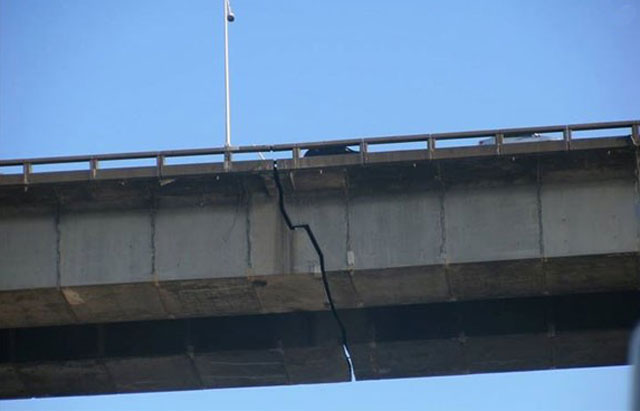
\includegraphics[width=5cm]{images/crack.jpg}
		\end{center}
		\end{column}
		\begin{column}{0.7\textwidth}
		\begin{center}
			\pause
			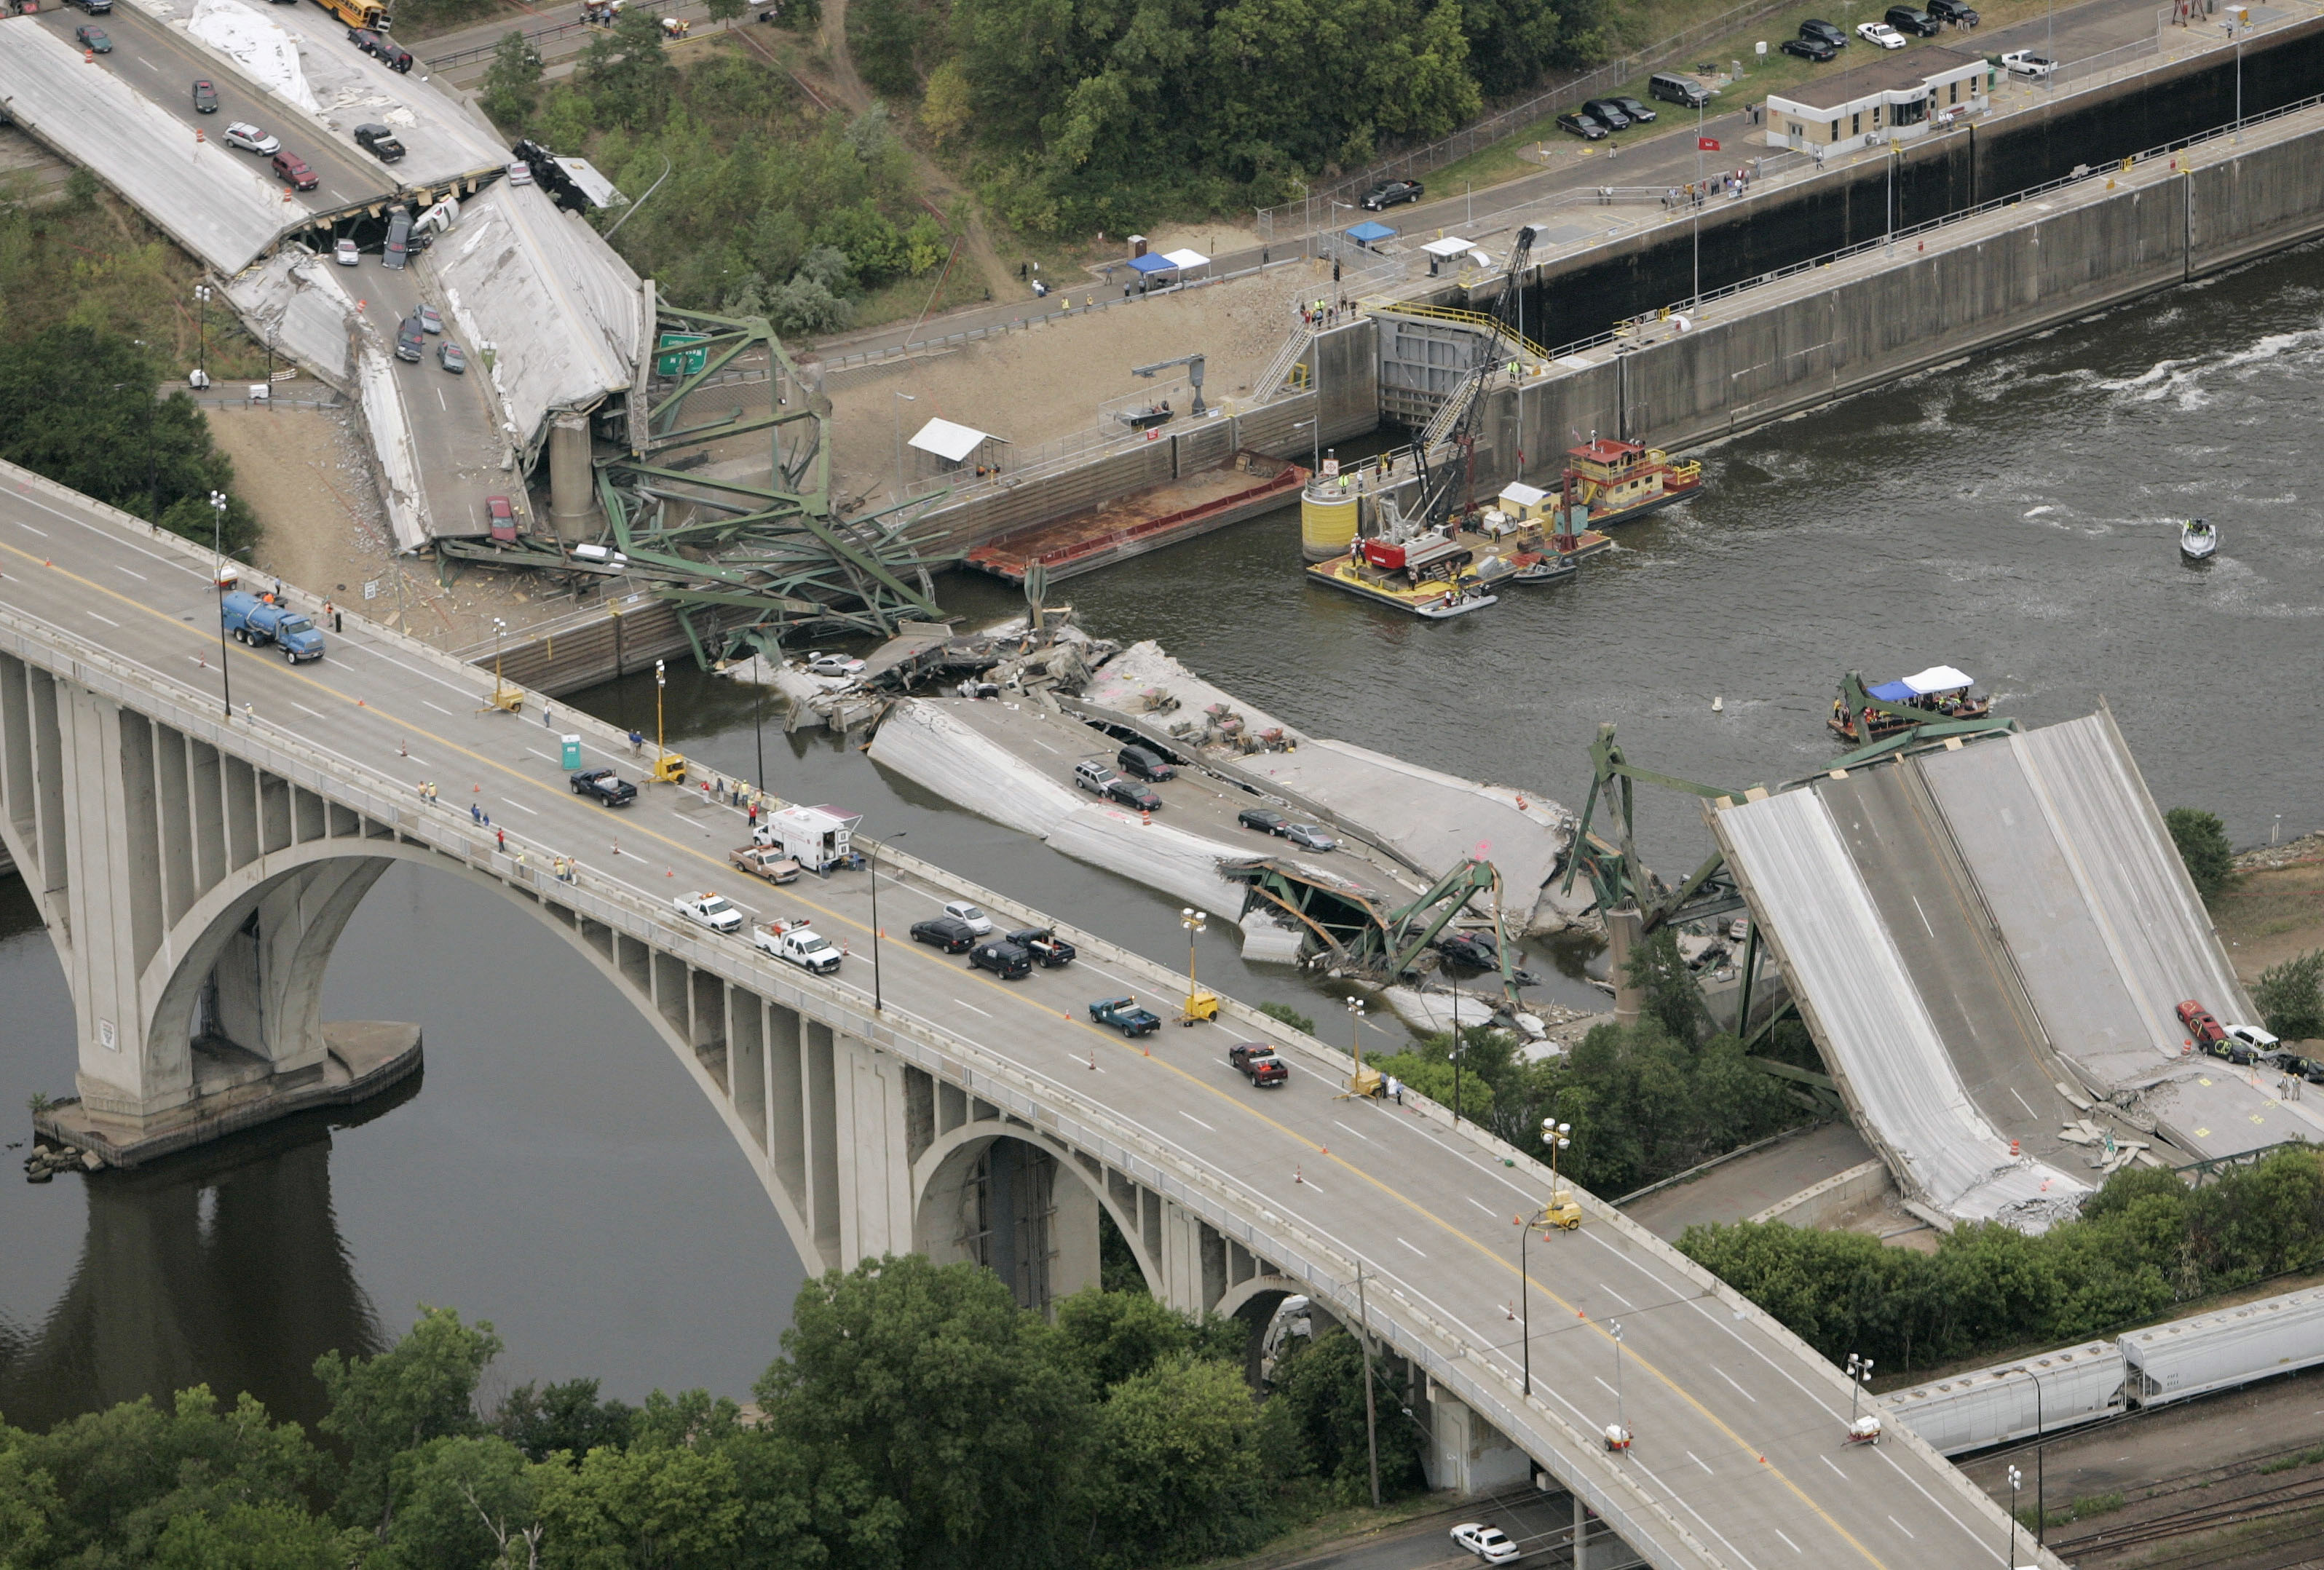
\includegraphics[width=6cm]{images/minneapolis.jpg}
		\end{center}
		\end{column}
	\end{columns}

\vspace{1\baselineskip}
\begin{itemize}
\item ``Better safe than sorry."
\vspace{1\baselineskip}
\item Example: accelerate inspection of post-earthquake damage.
\end{itemize}
\end{frame}


\subsection{Definitions}

\begin{frame}{Definitions}
\begin{exampleblock}{Damages}
Changes in a system that negatively affect its performance.
\end{exampleblock}
\begin{center}
	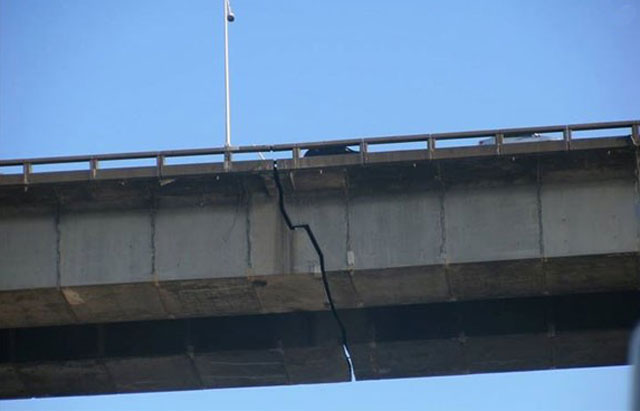
\includegraphics[width=4.5cm]{images/crack.jpg}
\end{center}
\begin{exampleblock}{Structure Health Monitoring}
A damage identification strategy for aerospace, civil and mechanical structures.
\end{exampleblock}

\end{frame}


\subsection{4 levels in damage identification}
\begin{frame}{4 levels in damage identification}

\begin{center}
\begin{itemize}[<+->]
\item Detection: Is the structure damaged or not?
\vspace{1\baselineskip}
\item Localization: Where is the damaged area located?
\vspace{1\baselineskip}
\item Quantification: What is the extent of damage?
\vspace{1\baselineskip}
\item Prediction: What is the remaining service life of the structure?
\end{itemize}
\end{center}
\end{frame}


\begin{frame}{transition/plan}
\end{frame}

%%%%%%%%%%%%%%%%%%%%%%%%%%%%%%%%%%%%%%%%%%%%%%%%%%%%%%%%%%%%%%%%%%%%%%%%%%%%%%%%%%%%%%%%%%%%%%%%%%%%%%%%%%%%%%%%%

\section{State of the art}


\begin{frame}{intro}
\end{frame}


\begin{frame}{Model based methods}
\end{frame}


\begin{frame}{Data driven methods}
\end{frame}


\begin{frame}{Combined methods}
\end{frame}


\begin{frame}{transition}
\end{frame}

%%%%%%%%%%%%%%%%%%%%%%%%%%%%%%%%%%%%%%%%%%%%%%%%%%%%%%%%%%%%%%%%%%%%%%%%%%%%%%%%%%%%%%%%%%%%%%%%%%%%%%%%%%%%%%%%%

\section{Physical Models}


\begin{frame}{Finite Elements model}

\begin{center}
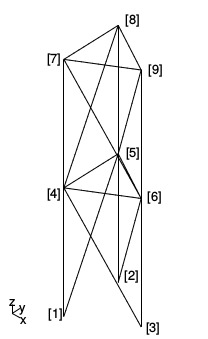
\includegraphics[height=4cm]{images/finite_element.png}

$M \ddot{q}(t) + C \dot{q}(t) + K q(t) = f(t)$
\end{center}

\end{frame}


\begin{frame}{Continous-time state-space model}
With the variable change $x =
\begin{pmatrix}
\dot{q} \\
q
\end{pmatrix}$, we have:


\begin{center}
$\left\{
\begin{array}{ll}
\dot{x}(t) = A_cx(t) + B_cf(t) \\
y(t) = C_cx(t) + D_cf(t)
\end{array}
\right.$
\end{center}

where $A_c, B_c, C_c$ and $D_c$ rely on $M, C$ and $K$.

\end{frame}


\begin{frame}{Discret-time state-space model}

We need to convert the system to discret time:

\begin{center}

$\left\{
\begin{array}{ll}
x_{k+1} & = A_dx_k + B_df_k \\
y_k & = C_dx_k + B_df_k
\end{array}
\right.$


\end{center}

where

\begin{center}


$\begin{array}{ll}
A_d = exp(A_c \Delta t) \\
B_d= (A_d - I) A^{-1}_c B_c \\
C_d = C_c \\
D_d = D_c
\end{array}$

\end{center}


\end{frame}
%%%%%%%%%%%%%%%%%%%%%%%%%%%%%%%%%%%%%%%%%%%%%%%%%%%%%%%%%%%%%%%%%%%%%%%%%%%%%%%%%%%%%%%%%%%%%%%%%%%%%%%%%%%%%%%%%

\section{FRF Interpolation Method}


\begin{frame}{FRF Interpolation Method}

\begin{alertblock}{Main hypothesis}
A concentrated damage reflects
in a loss of spatial regularity of the vibrational profile of a
structure, compared with the undamaged state.
\end{alertblock}


\underline{Main steps}:
\begin{itemize}
\item Frequency Response Function (FRF) calcul
\item Interpolation on the FRF
\item Error calcul
\end{itemize}


\end{frame}


\begin{frame}{Interpolation}
Cubic polynomial spline interpolation:

\begin{center}
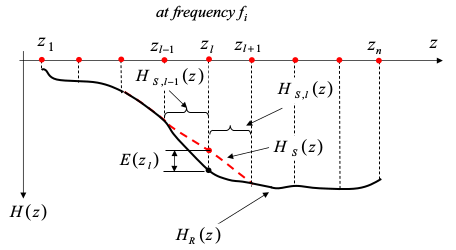
\includegraphics[width=5cm]{images/interpolation.png}
\end{center}

\end{frame}


\begin{frame}{Error calcul}

For each sensor $z_l$ at the frequency $f_i$:
\begin{center}
$E(z_l,f_i) = | H_R(z_l,f_i) - H_S(z_l,f_i) |$
\end{center}


For each sensor:
\begin{center}
$E(z_l) = \sqrt{  \sum\limits_{i=1}^N  E^2(z_l,f_i) }$
\end{center}


Difference with the reference state:
\begin{center}
$\Delta E(z_l) = E_d(z_l) - E_0(z_l)$
\end{center}

\end{frame}

\begin{frame}{Probability of identification of a damage}
\begin{center}
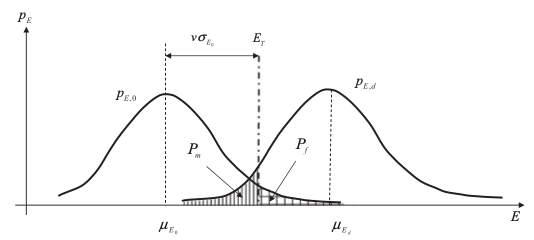
\includegraphics[height=4cm]{images/gaussiennes.png}
\end{center}
\end{frame}

%%%%%%%%%%%%%%%%%%%%%%%%%%%%%%%%%%%%%%%%%%%%%%%%%%%%%%%%%%%%%%%%%%%%%%%%%%%%%%%%%%%%%%%%%%%%%%%%%%%%%%%%%%%%%%%%%

\section{Simulation}

\begin{frame}{System masses-springs}
\begin{center}
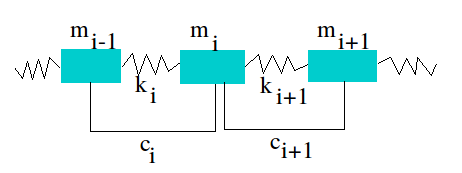
\includegraphics[width=5cm]{images/ressorts.png}

$M \ddot{q}(t) + C \dot{q}(t) + K q(t) = f(t)$
\end{center}




\end{frame}


\begin{frame}{Sample frequency and Discret-time state-space model}

We find the sample frequency with the eigenvalues of the matrix $A_c$ of the continous-time state-space model.

\vspace{5mm}

Thus, we have the matrices of the discrete-time state-space model:
\begin{center}
$\left\{
\begin{array}{ll}
x_{k+1} & = A_dx_k + B_df_k \\
y_k & = C_dx_k + B_df_k
\end{array}
\right.$
\end{center}

\end{frame}

\begin{frame}{FRF and Interpolation}
\end{frame}

\begin{frame}{Results}
\begin{center}
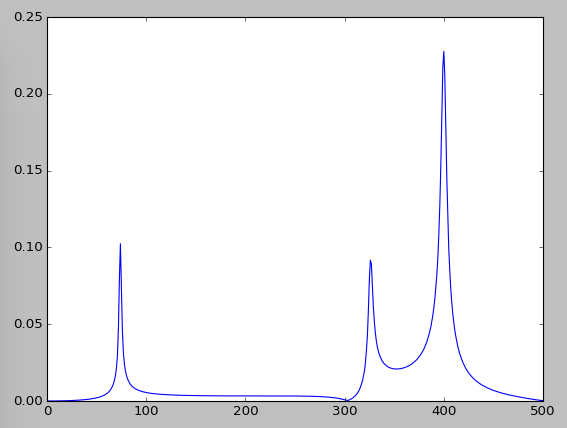
\includegraphics[width=5cm]{images/FRF_freq.png}

FRF for one sensor in function of frequencies
\end{center}
\end{frame}

\begin{frame}{Results}
\begin{center}
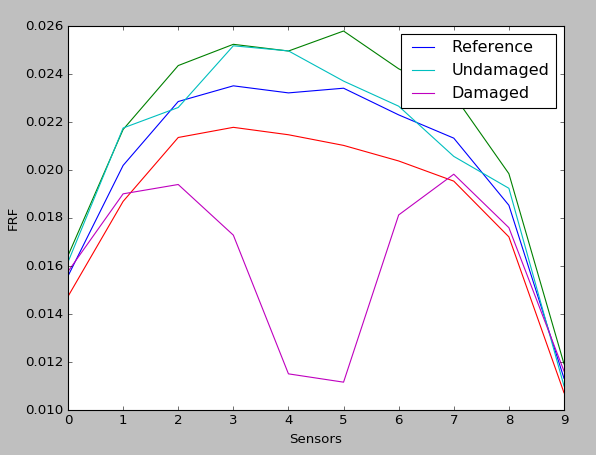
\includegraphics[width=5cm]{images/curve_damage.png}

For a fixed frequency, the FRF value for each sensor
\end{center}

\end{frame}

\begin{frame}{Results}
\end{frame}


%%%%%%%%%%%%%%%%%%%%%%%%%%%%%%%%%%%%%%%%%%%%%%%%%%%%%%%%%%%%%%%%%%%%%%%%%%%%%%%%%%%%%%%%%%%%%%%%%%%%%%%%%%%%%%%%%

\section{Conclusion}

\begin{frame}{Conclusion}
\end{frame}


  \end{document}
